\documentclass{article}

\usepackage[utf8]{inputenc}
\usepackage[dvipsnames]{xcolor}
\usepackage{lmodern}
\usepackage{graphicx}
\usepackage{longtable}
\usepackage{tabularx}
\graphicspath{ {../images/} }
\usepackage{imakeidx}
\makeindex[columns=3, title=Alphabetical Index, intoc]

\usepackage{tabularx}
\usepackage{amsmath}
\usepackage{paralist}
\usepackage{enumitem}
\usepackage{hyperref} %\usepackage[hidelinks]{hyperref} %per togliere bordi rossi
\usepackage{makecell}
\usepackage{caption}
\usepackage[maxfloats=256]{morefloats}
\maxdeadcycles=1000

\usepackage[official]{eurosym}
\DeclareUnicodeCharacter{20AC}{\euro{}}

\author{Agosta, Belli, Emili, Giacchini, Luciani}

\begin{document}

\begin{center}
    \sffamily{\fontsize{50}{48} \selectfont \textcolor{red}{Nexi}\textcolor{green}{Fy}}
\end{center}

\begin{center}
    \itshape{\fontsize{20}{48} \selectfont streaming to your pocket}
\end{center}

\bigskip\bigskip\bigskip

\begin{flushleft}
    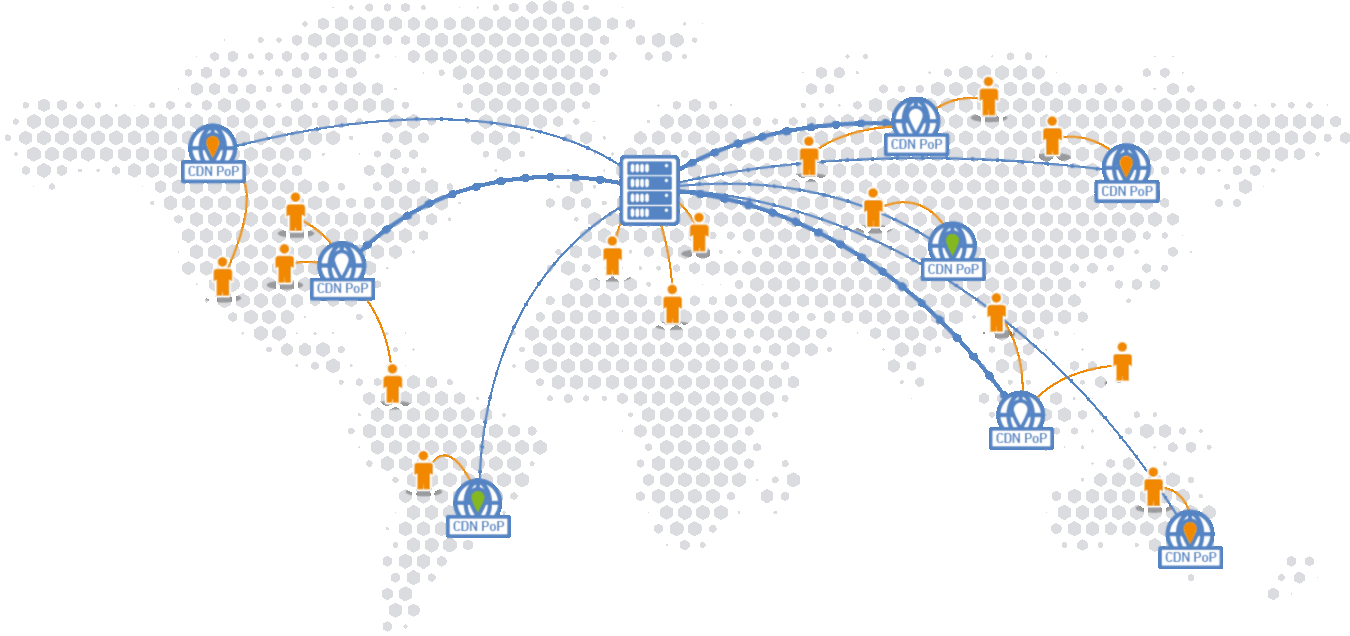
\includegraphics[scale=1]{../images/worldCDN.png}
\end{flushleft}

\bigskip\bigskip\bigskip

\begin{center}
    \itshape{\fontsize{30}{48} \selectfont Piano dei test}
\end{center}

\newpage
\printindex

\newpage
\section{\itshape{Piano dei test}}
\subsection*{Tipologia}
I test saranno effettuati in due diverse tipologie:
\begin{itemize}
    \item Black box: valutano le funzionalità dell'applicazione a partire dall'interfaccia utente, che
          sia quella degli amministratori o degli utenti fruitori del servizio. Quindi si ignorano le dinamiche
          interne al sistema. Contengono anche test di esperienza e usabilità utente, ovvero quelli che richiedono
          un interazione umana.
    \item White box: provano la correttezza del sistema con test unitari sui suoi componenti interni,
          così come le interazioni tra i vari componenti.
\end{itemize}

\subsection*{Ambiente di test}
Per i test di tipo White Box vengono definiti i seguenti programmi di supporto:
\begin{itemize}
    \item Un programma per intercettare le comunicazioni client-server e server-server, per controllare che le
          comunicazioni avvengano in modo corretto;
    \item Un programma per verificare lo stato ed il contenuto del database;
    \item Un profiler per controllare lo stato delle performance e verificare l’assenza di colli di bottiglia;
\end{itemize}
L’ambiente viene re-inizializzato per ogni test, in quanto eseguito su un container.

\subsection*{Dati su cui vengono eseguiti i test}

\subsubsection*{Dati non presenti nel database}
\begin{itemize}
    \item Token autenticazione auth\_t\_wrong
    \item Nome abbonamento nome\_abb\_nv
    \item Nome abbonamento nome\_abb\_v
    \item Prezzo abbonamento prezzo\_abb\_v
    \item Prezzo abbonamento prezzo\_abb\_nv
    \item Durata abbonamento duarata\_abb\_v
    \item Durata abbonamento duarata\_abb\_nv

\end{itemize}

\subsubsection*{Dati presenti nel database}
\begin{itemize}
    \item Token autenticazione amministratore auth\_admin\_t
    \item Token autenticazione auth\_t
    \item PianoDiAbbonamento piano\_abb
    \item PianoDiAbbonamento piano\_abb\_full
    \item PianoDiAbbonamento piano\_abb\_empty
    \item Utente utente

\end{itemize}

\subsection*{Descrizione priorità dei test}

Vengono definite le seguenti priorità per classificare i vari test in base a quanto importante sia la
loro corretta e periodica esecuzione sull'integrità del sistema.
\begin{itemize}
    \item H (alta priorità): relativa ai test che devono essere eseguiti correttamente per garantire l'integrità
          del sistema;
    \item M (media priorità): relativa ai test che devono essere eseguiti correttamente per garantire l'integrità
          del sistema, ma solo successivamente ai test di priorità H;
    \item L (bassa priorità): relativa ai test che possono essere eseguiti, per garantire una migliore funzionalità
          del sistema, ma solo successivamente ai test di priorità M.
\end{itemize}


\begin{longtable}{| p{.10\textwidth} | p{.70\textwidth} | p{.14\textwidth} |}
    \caption{Casi d'uso}                                                         \\
    \hline
    \textbf{ID TEST} & \textbf{ID UC}                        & \textbf{Priorità} \\\hline
    T\_1             & UC\_GestisciAbbonamenti               & H                 \\\hline
    T\_2             & UC\_CreaAbbonamento                   & H                 \\\hline
    T\_3             & UC\_RecuperaAbbonamentiEsistenti      & M                 \\\hline
    T\_4             & UC\_RecuperaServizi                   & M                 \\\hline
    T\_5             & UC\_DisattivaAbbonamento              & H                 \\\hline
    T\_6             & UC\_AggiungiServizioAbbonamento       & H                 \\\hline
    T\_7             & UC\_RimuoviServizioAbbonamento        & H                 \\\hline
    T\_8             & UC\_RecuperaServiziAbbonamento        & M                 \\\hline
    T\_9             & UC\_RecuperaPianiAbbonamentoUtente    & M                 \\\hline
    T\_10            & UC\_EffettuaPagamentoPartner          & H                 \\\hline
    T\_11            & UC\_CalcolaImportoDaPagare            & H                 \\\hline
    T\_12            & UC\_GestisciSottoscrizioniAbbonamenti & H                 \\\hline
    T\_13            & UC\_SottoscriviAbbonamento            & H                 \\\hline
    T\_14            & UC\_DisdiciAbbonamento                & H                 \\\hline
    T\_15            & UC\_CambiaAbbonamento                 & H                 \\\hline
    T\_16            & UC\_GestisciScadenzeAbbonamenti       & H                 \\\hline
    T\_17            & UC\_SospendiAccount                   & M                 \\\hline
    T\_18            & UC\_RiattivaAccount                   & M                 \\\hline
    T\_19            & UC\_RiattivaAccountAutomatico         & H                 \\\hline
    T\_20            & UC\_EffettuaRegistrazione             & H                 \\\hline
    T\_21            & UC\_ModificaProfilo                   & L                 \\\hline
    T\_22            & UC\_EffettuaLogin                     & M                 \\\hline
    T\_23            & UC\_EffettuaLogout                    & M                 \\\hline
    T\_24            & UC\_OttieniCronologia                 & L                 \\\hline
    T\_25            & UC\_GestisciProdotti                  & H                 \\\hline
    T\_26            & UC\_CreaProdotto                      & H                 \\\hline
    T\_27            & UC\_ModificaInformazioniDiBase        & M                 \\\hline
    T\_28            & UC\_CaricaFile                        & H                 \\\hline
    T\_29            & UC\_CambiaVisibilitàProdotto          & M                 \\\hline
    T\_30            & UC\_RiproduciProdotto                 & M                 \\\hline
    T\_31            & UC\_StreamingVideo                    & M                 \\\hline
    T\_32            & UC\_StreamingMusica                   & M                 \\\hline
    T\_33            & UC\_PausaPlayer                       & M                 \\\hline
    T\_34            & UC\_SpostaPuntoRiproduzionePlayer     & M                 \\\hline
    T\_35            & UC\_DownloadProdotto                  & M                 \\\hline
    T\_36            & UC\_VisualizzaPubblicità              & M                 \\\hline
    T\_37            & UC\_RiproduciAudioInBackground        & M                 \\\hline
    T\_38            & UC\_SegnalaProdotto                   & M                 \\\hline
    T\_39            & UC\_GestisciSegnalazioni              & H                 \\\hline
    T\_40            & UC\_OttieniSegnalazioni               & M                 \\\hline
    T\_41            & UC\_ChiudiSegnalazione                & M                 \\\hline
    T\_42            & UC\_RiapriSegnalazione                & M                 \\\hline
    T\_43            & UC\_VisualizzaProdottoSegnalato       & M                 \\\hline
    T\_44            & UC\_RicercaContenuto                  & M                 \\\hline
    T\_45            & UC\_RicercaPopolari                   & L                 \\\hline
    T\_46            & UC\_SuggerisciContenuti               & M                 \\\hline
    T\_47            & UC\_GestisciPlaylist                  & H                 \\\hline
    T\_48            & UC\_CreaPlaylist                      & M                 \\\hline
    T\_49            & UC\_AggiungiProdottoPlaylist          & M                 \\\hline
    T\_50            & UC\_RimuoviProdottoPlaylist           & M                 \\\hline
    T\_51            & UC\_CambiaVisibilitàPlaylist          & M                 \\\hline
    T\_52            & UC\_RiproduciPlaylist                 & M                 \\\hline
    T\_53            & UC\_CreaSerieTv                       & H                 \\\hline
    T\_54            & UC\_CreaAlbum                         & H                 \\\hline
    T\_55            & UC\_AggiungiProdottoAllaCoda          & M                 \\\hline
    T\_56            & UC\_RimuoviProdottoDallaCoda          & M                 \\\hline
    T\_57            & UC\_MostraStatoCoda                   & L                 \\\hline
    T\_58            & UC\_RiproduciCoda                     & M                 \\\hline
    T\_59            & UC\_CalcolaQualitàContenuto           & M                 \\\hline
    T\_60            & UC\_VotaContenuto                     & L                 \\\hline
    T\_61            & UC\_CommentaContenuto                 & L                 \\\hline
    T\_62            & UC\_RimuoviCommento                   & L                 \\\hline
    T\_63            & UC\_AttivaAbbonamento                 & H                 \\\hline
\end{longtable}

\subsection*{Realizzazione dei test}

\begin{table}[hb]
    \centering
    \begin{tabular}{ |p{2cm}|p{10cm}|  }
        \hline
        ID          & T\_1                                                                   \\\hline
        Caso d'uso  & UC\_GestisciAbbonamenti                                                \\\hline
        Obbiettivo  & Testare l'interfaccia per la gestione dei piani di abbonamento         \\\hline
        Prerequsiti & La persona è autenticata nel sistema ed ha privilegi di Amministratore \\\hline
        Tipologia   & White box                                                              \\\hline
        Azioni      &
        TEST1:
        \begin{enumerate}[nosep, topsep=0pt]
            \item richiedere la visualizzazione della gestione abbonamenti, fornendo il token di autenticazione \emph{auth\_t\_wrong};
            \item verificare che il sistema restituisca errore di permesso negato;
        \end{enumerate}
        \vspace{0.5cm} TEST2:
        \begin{enumerate}[nosep, topsep=0pt]
            \item richiedere la visualizzazione della gestione abbonamenti, fornendo il token di autenticazione \emph{auth\_t};
            \item verificare che il sistema restituisca errore di permesso negato;
        \end{enumerate}
        \vspace{0.5cm}TEST3:
        \begin{enumerate}[nosep, topsep=0pt]
            \item richiedere la visualizzazione della gestione abbonamenti, fornendo il token di autenticazione \emph{auth\_admin\_t};
            \item verificare che il sistema restituisca la pagina con la lista di abbonamenti richiesti;
        \end{enumerate}
        \\\hline
    \end{tabular}
\end{table}

\begin{table}[hb]
    \centering
    \begin{tabular}{ |p{2cm}|p{10cm}|  }
        \hline
        ID          & T\_2                                                                                                                                \\\hline
        Caso d'uso  & UC\_CreaAbbonamento                                                                                                                 \\\hline
        Obbiettivo  & Testare la creazione di un nuovo piano di abbonamento                                                                               \\\hline
        Prerequsiti & Il sistema permette di inserire nuovi piani di abbonamento e la persona è autenticata nel sistema ed ha privilegi di Amministratore \\\hline
        Tipologia   & White box                                                                                                                           \\\hline
        Azioni      &
        TEST1:
        \begin{enumerate}[nosep, topsep=0pt]
            \item fornire i seguenti valori \emph{nome\_abb\_nv}, \emph{prezzo\_abb\_nv}, \emph{durata\_abb\_nv};
            \item verifica che il sistema restituisca errore nella validazione dei dati;
        \end{enumerate}
        \vspace{0.5cm} TEST2:
        \begin{enumerate}[nosep, topsep=0pt]
            \item fornire i seguenti valori \emph{nome\_abb\_nv}, \emph{prezzo\_abb\_v}, \emph{durata\_abb\_v};
            \item verifica che il sistema restituisca errore nell'inserimento di un piano di abbonamento duplicato;
        \end{enumerate}
        \vspace{0.5cm} TEST3:
        \begin{enumerate}[nosep, topsep=0pt]
            \item fornire i seguenti valori \emph{nome\_abb\_v}, \emph{prezzo\_abb\_v}, \emph{durata\_abb\_v};
            \item verifica che il sistema restituisca errore generico nella crezione di un abbonamento oppure creazione effettuata correttamente;
        \end{enumerate}
        \\\hline
    \end{tabular}
\end{table}

\begin{table}[hb]
    \centering
    \begin{tabular}{ |p{2cm}|p{10cm}|  }
        \hline
        ID          & T\_3                                                                               \\\hline
        Caso d'uso  & UC\_RecuperaAbbonamentiEsistenti                                                   \\\hline
        Obbiettivo  & Testare che tutti i piani di abbonamenti esistenti sono recuperati                 \\\hline
        Prerequsiti & La persona è autenticata nel sistema ed ha privilegi di Amministratore o di Utente \\\hline
        Tipologia   & Black box                                                                          \\\hline
        Azioni      &
        TEST1:
        \begin{enumerate}[nosep, topsep=0pt]
            \item richiedere di visualizzare la lista degli abbonamenti esistenti;
            \item verificare che vengano mostrati tutti gli abbonamenti esistenti;
        \end{enumerate}
        \\\hline
    \end{tabular}
\end{table}

\begin{table}[hb]
    \centering
    \begin{tabular}{ |p{2cm}|p{10cm}|  }
        \hline
        ID          & T\_4                                                                   \\\hline
        Caso d'uso  & UC\_RecuperaServizi                                                    \\\hline
        Obbiettivo  & Testare che tutti i servizi esistenti sono recuperati                  \\\hline
        Prerequsiti & La persona è autenticata nel sistema ed ha privilegi di Amministratore \\\hline
        Tipologia   & Black box                                                              \\\hline
        Azioni      &
        TEST1:
        \begin{enumerate}[nosep, topsep=0pt]
            \item richiedere di visualizzare la lista degli servizi esistenti;
            \item verificare che vengano mostrati tutti i servizi esistenti;
        \end{enumerate}
        \\\hline
    \end{tabular}
\end{table}

\begin{table}[hb]
    \centering
    \begin{tabular}{ |p{2cm}|p{10cm}|  }
        \hline
        ID          & T\_5                                                                   \\\hline
        Caso d'uso  & UC\_DisattivaAbbonamento                                               \\\hline
        Obbiettivo  & Testare che un abbonamento non sia più sottoscrivibile                 \\\hline
        Prerequsiti & La persona è autenticata nel sistema ed ha privilegi di Amministratore \\\hline
        Tipologia   & Black box                                                              \\\hline
        Azioni      &
        TEST1:
        \begin{enumerate}[nosep, topsep=0pt]
            \item richiedere la disattivazione di \emph{piano\_abb}
            \item verificare che il sistema ritorni il messaggio di avvenuta disattivazione dell'abbonamento;
        \end{enumerate}
        \\\hline
    \end{tabular}
\end{table}

\begin{table}[hb]
    \centering
    \begin{tabular}{ |p{2cm}|p{10cm}|  }
        \hline
        ID          & T\_6                                                                               \\\hline
        Caso d'uso  & UC\_AggiungiServizioAbbonamento                                                    \\\hline
        Obbiettivo  & Testare l'aggiunta del servizio di abbonamento al piano di abbonamento specificato \\\hline
        Prerequsiti & La persona è autenticata nel sistema ed ha privilegi di Amministratore             \\\hline
        Tipologia   & White box                                                                          \\\hline
        Azioni      &
        TEST1:
        \begin{enumerate}[nosep, topsep=0pt]
            \item fornire un piano di abbonamento \emph{piano\_abb\_full};
            \item verificare che il sistema mostri l'errore "Il piano possiede già tutti i servizi";
        \end{enumerate}
        \vspace{0.5cm} TEST2:
        \begin{enumerate}[nosep, topsep=0pt]
            \item fornire un piano di abbonamento \emph{piano\_abb};
            \item verifica che il sistema restituisca la lista di servizi \emph{L} che possono essere aggiunti;
            \item fornire il servizio richiesto scegliendolo da \emph{L};
            \item verificare che il sistema mostri un errore generico oppure modifica effettuata con successo;
        \end{enumerate}
        \\\hline
    \end{tabular}
\end{table}

\begin{table}[hb]
    \centering
    \begin{tabular}{ |p{2cm}|p{10cm}|  }
        \hline
        ID          & T\_7                                                                                  \\\hline
        Caso d'uso  & UC\_RimuoviServizioAbbonamento                                                        \\\hline
        Obbiettivo  & Testare la rimozione del servizio di abbonamento dal piano di abbonamento specificato \\\hline
        Prerequsiti & La persona è autenticata nel sistema ed ha privilegi di Amministratore                                                                                     \\\hline
        Tipologia   & White box                                                                             \\\hline
        Azioni      &
        TEST1:
        \begin{enumerate}[nosep, topsep=0pt]
            \item fornire un piano di abbonamento \emph{piano\_abb\_empty};
            \item verificare che il sistema mostri l'errore "Non ci sono servizi da rimuovere";
        \end{enumerate}
        \vspace{0.5cm} TEST2:
        \begin{enumerate}[nosep, topsep=0pt]
            \item fornire un piano di abbonamento \emph{piano\_abb};
            \item verifica che il sistema restituisca la lista di servizi \emph{L} che possono essere rimossi;
            \item fornire il servizio richiesto scegliendolo da \emph{L};
            \item verificare che il sistema mostri un errore generico oppure modifica effettuata con successo;
        \end{enumerate}
        \\\hline
    \end{tabular}
\end{table}

\begin{table}[hb]
    \centering
    \begin{tabular}{ |p{2cm}|p{10cm}|  }
        \hline
        ID          & T\_8                                                                                       \\\hline
        Caso d'uso  & UC\_RecuperaServiziAbbonamento                                                             \\\hline
        Obbiettivo  & Testare il recupero di tutti i servizi di abbonamento associati ad un piano di abbonamento \\\hline
        Prerequsiti & La persona è autenticata nel sistema ed ha privilegi di Amministratore o di Utente                                                                                          \\\hline
        Tipologia   & Black box                                                                                  \\\hline
        Azioni      &
        TEST1:
        \begin{enumerate}[nosep, topsep=0pt]
            \item fornire un piano di abbonamento \emph{piano\_abb};
            \item verificare che vengano mostrati tutti i servizi esistenti associati al piano di abbonamento specificato;
        \end{enumerate}
        \vspace{0.5cm} TEST2:
        \begin{enumerate}[nosep, topsep=0pt]
            \item fornire un piano di abbonamento \emph{piano\_abb\_empty};
            \item verificare la lista dei servizi restituita sia vuota;
        \end{enumerate}
        \\\hline
    \end{tabular}
\end{table}

\begin{table}[hb]
    \centering
    \begin{tabular}{ |p{2cm}|p{10cm}|  }
        \hline
        ID          & T\_9                                                                           \\\hline
        Caso d'uso  & UC\_RecuperaPianiAbbonamentoUtente                                             \\\hline
        Obbiettivo  & Testare che la lista degli abbonamenti restituita sia quella degli abbonamenti
        sottoscritti dall'utente                                                                     \\\hline
        Prerequsiti & La persona è autenticata nel sistema ed ha privilegi di Amministratore e \emph{utente} è un utente attivo                                               \\\hline
        Tipologia   & Black box                                                                      \\\hline
        Azioni      &
        TEST1:
        \begin{enumerate}[nosep, topsep=0pt]
            \item richiedere lista \emph{L} piani di abbonamento sottoscritti da \emph{utente};
            \item verificare che \emph{L} sia la lista degli abbonamenti sottoscritti da \emph{utente};
        \end{enumerate}
        \\\hline
    \end{tabular}
\end{table}

\begin{table}[hb]
    \centering
    \begin{tabular}{ |p{2cm}|p{10cm}|  }
        \hline
        ID          & T\_10                                                             \\\hline
        Caso d'uso  & UC\_EffettuaPagamentoPartner                                      \\\hline
        Obbiettivo  & Verificare che il pagamento verso i partner avvenga correttamente \\\hline
        Prerequsiti & Il processo ha privilegi di Amministratore                                                                 \\\hline
        Tipologia   & White box                                                         \\\hline
        Azioni      &
        TEST1:
        \begin{enumerate}[nosep, topsep=0pt]
            \item richiedere la lista di tutti gli utenti \emph{LU};
            \item verificare che \emph{LU} sia la lista di tutti gli utenti;
            \item tra tutti gli utenti in \emph{LU}, controllare tutti coloro che
                  hanno un servizio per pubblicare prodotti e salvarli in \emph{LP};
            \item verificare che \emph{LP} sia la lista di tutti gli utenti che
                  hanno un servizio per pubblicare prodotti;
            \item per ogni utente \emph{U} in \emph{LP}:
                  \begin{itemize}
                      \item ottenere coordinate le bancarie \emph{CB} di \emph{U}
                      \item controllare che \emph{CB} siano valide
                      \item ottenere l'importo da pagare \emph{I}
                      \item effettuare pagamento verso \emph{CB} attraverso il sistema
                            di pagamento.
                      \item controllare che se il pagamento è andato a buon fine, venga aggiornato il giorno di
                            pagamento utente e inviata una mail con messaggio di avvenuto pagamento a \emph{U}
                      \item controllare che se il pagamento non è andato a buon fine, venga inviata una mail
                            con messaggio di errore a \emph{U}
                  \end{itemize}

        \end{enumerate}
        \\\hline
    \end{tabular}
\end{table}

\begin{table}[hb]
    \centering
    \begin{tabular}{ |p{2cm}|p{10cm}|  }
        \hline
        ID          & T\_11                                                                             \\\hline
        Caso d'uso  & UC\_CalcolaImportoDaPagare                                                        \\\hline
        Obbiettivo  & Testare il corretto funzionamento del calcolo dell'importo da pagare ad un utente \\\hline
        Prerequsiti & \emph{utente} è un utente attivo                                                  \\\hline
        Tipologia   & White box                                                                         \\\hline
        Azioni      &
        TEST1:
        \begin{enumerate}[nosep, topsep=0pt]
            \item richiedere il calcolo dell'importo dovuto, fornendo \emph{utente};
            \item verificare che il sistema consideri l'intervallo di tempo [\emph{DA}, \emph{A}], dove \emph{DA} è null sse non esistono pagamenti precedenti verso quell'utente;
            \item verificare che il sistema consideri la lista dei prodotti relativa ad \emph{utente} e che il totale dovuto \emph{TOT} sia initializzato a 0;
            \item verificare che il sistema ritorni \emph{R = TOT + V}, con V il numero complessivo di visualizzazioni, assieme alla funzione \emph{F} che indica come calcolare l'importo da pagare a partire da \emph{R};
        \end{enumerate}
        \\\hline
    \end{tabular}
\end{table}

\begin{table}[hb]
    \centering
    \begin{tabular}{ |p{2cm}|p{10cm}|  }
        \hline
        ID          & T\_12                                                                               \\\hline
        Caso d'uso  & UC\_GestisciSottoscrizioniAbbonamenti                                               \\\hline
        Obbiettivo  & Testare l'interfaccia per la gestione delle sottoscrizioni dei piani di abbonamento \\\hline
        Prerequsiti & -                                                                                   \\\hline
        Tipologia   & White box                                                                           \\\hline
        Azioni      &
        TEST1:
        \begin{enumerate}[nosep, topsep=0pt]
            \item richiedere la visualizzazione della gestione delle sottoscrizioni dei piani di abbonamento, fornendo il token di autenticazione \emph{auth\_t\_wrong};
            \item verificare che il sistema restituisca errore di permesso negato;
        \end{enumerate}
        \vspace{0.5cm} TEST2:
        \begin{enumerate}[nosep, topsep=0pt]
            \item richiedere la visualizzazione della gestione delle sottoscrizioni dei piani di abbonamento, fornendo il token di autenticazione \emph{auth\_t};
            \item verificare che il sistema restituisca la pagina con la lista delle sottoscrizioni richieste;
        \end{enumerate}
        \\\hline
    \end{tabular}
\end{table}

\begin{table}[hb]
    \centering
    \begin{tabular}{ |p{2cm}|p{10cm}|  }
        \hline
        ID          & T\_13                                                             \\\hline
        Caso d'uso  & UC\_SottoscriviAbbonamento                                        \\\hline
        Obbiettivo  & Testare la sottoscrizione di un abbonamento da parte di un utente \\\hline
        Prerequsiti & -                                                                 \\\hline
        Tipologia   & White box                                                         \\\hline
        Azioni      &
        TEST1:
        \begin{enumerate}[nosep, topsep=0pt]
            \item richiedere la sottoscrizione di un abbonamento, fornendo \emph{piano\_abb} e le coordinate bancarie \emph{CB} dell'utente;
            \item verificare che il pagamento venga registrato;
            \item verificare che l'abbonamento venga aggiunto alle sottoscrizioni dell'utente oppure che il sistema restituisca un errore durante l'aggiunta dell'abbonamento;
        \end{enumerate}
        \\\hline
    \end{tabular}
\end{table}

\begin{table}[hb]
    \centering
    \begin{tabular}{ |p{2cm}|p{10cm}|  }
        \hline
        ID          & T\_14                                                                                              \\\hline
        Caso d'uso  & UC\_DisdiciAbbonamento                                                                             \\\hline
        Obbiettivo  & Testare la disdetta di un piano di abbonamento e la relativa disattivazione del rinnovo automatico \\\hline
        Prerequsiti & \emph{piano\_abb} è un piano di abbonamento attivo dell'utente corrente                            \\\hline
        Tipologia   & White box                                                                                          \\\hline
        Azioni      &
        TEST1:
        \begin{enumerate}[nosep, topsep=0pt]
            \item richiedere la disdetta di un piano di abbonamento, fornendo \emph{piano\_abb};
            \item verificare che il sistema disattivi il rinnovo automatico di \emph{piano\_abb};
            \item verificare che il sistema ritorni la pagina mostrando "Cambiamento avvenuto con successo" oppure "Errore Generico";
        \end{enumerate}
        \\\hline
    \end{tabular}
\end{table}

\begin{table}[hb]
    \centering
    \begin{tabular}{ |p{2cm}|p{10cm}|  }
        \hline
        ID          & T\_15                                                                                       \\\hline
        Caso d'uso  & UC\_CambiaAbbonamento                                                                       \\\hline
        Obbiettivo  & Testare il corretto funzionamento del cambio di piano di abbonamento associato ad un utente \\\hline
        Prerequsiti & \emph{piano\_abb} è un piano di abbonamento attivo dell'utente corrente                     \\\hline
        Tipologia   & White box                                                                                   \\\hline
        Azioni      &
        TEST1:
        \begin{enumerate}[nosep, topsep=0pt]
            \item richiedere il cambiamento di un piano di abbonamento, fornendo \emph{piano\_abb};
            \item verificare che il sistema ritorni tutti i piani di abbonamento sottoscrivibili \emph{L} e che \emph{piano\_abb} non sia contenuto in \emph{L};
            \item fornire al sistema un piano di abbonamento \emph{P2} con prezzo \emph{PRICE2} $\geq$ \emph{PRICE}, dove \emph{PRICE} è il prezzo di \emph{piano\_abb};
            \item verificare che il sistema calcoli l'importo di pagamento \emph{R = PRICE2 - PRICE $\geq$ 0};
            \item fornire le coordinate bancarie \emph{CB} per procedere al pagamento;
            \item verificare che il sistema processi correttamente il pagamento e che l'importo \emph{R} venga correttamente accreditato;
            \item verificare che il sistema registri il pagamento effettuato e che \emph{piano\_abb} venga sostituito col piano di abbonamento \emph{P2};
            \item verificare che il sistema mostri la pagina di cambiamento effettuato oppure di errore generico;
        \end{enumerate}
        \vspace{0.5cm} TEST2:
        \begin{enumerate}[nosep, topsep=0pt]
            \item richiedere il cambiamento di un piano di abbonamento, fornendo \emph{piano\_abb};
            \item verificare che il sistema ritorni tutti i piani di abbonamento sottoscrivibili \emph{L} e che \emph{piano\_abb} non sia contenuto in \emph{L};
            \item fornire al sistema un piano di abbonamento \emph{P2} con prezzo \emph{PRICE2} $<$ \emph{PRICE}, dove \emph{PRICE} è il prezzo di \emph{piano\_abb};
            \item verificare che il sistema calcoli l'importo di pagamento \emph{R = 0};
            \item fornire le coordinate bancarie \emph{CB} per procedere al pagamento;
            \item verificare che il sistema processi correttamente il pagamento e che l'importo \emph{R} venga correttamente accreditato;
            \item verificare che il sistema registri il pagamento effettuato e che \emph{piano\_abb} venga sostituito col piano di abbonamento \emph{P2};
            \item verificare che il sistema mostri la pagina di cambiamento effettuato oppure di errore generico;
        \end{enumerate}
        \\\hline
    \end{tabular}
\end{table}

\begin{table}[hb]
    \centering
    \begin{tabular}{ |p{2cm}|p{10cm}|  }
        \hline
        ID          & T\_16                                                                                                              \\\hline
        Caso d'uso  & UC\_GestisciScadenzeAbbonamenti                                                                                    \\\hline
        Obbiettivo  & Testare il corretto funzionamento della gestione di un piano di abbonamento in scadenza                            \\\hline
        Prerequsiti & Il processo ha privilegi di Amministratore \\\hline
        Tipologia   & White box                                                                                                          \\\hline
        Azioni      &
        TEST1:
        \begin{enumerate}[nosep, topsep=0pt]
            \item verificare che il sistema consideri le sole sottoscrizioni in scadenza nella giornata corrente;
            \item per ogni sottoscrizione \emph{S}, verificare che:
                  \begin{itemize}
                      \item se \emph{S} è ancora sottoscrivibile ed è attivo il rinnovo automatico, allora il sistema processi il pagamento per il rinnovo di \emph{S}. Verificare inoltre che \emph{S} sia rinnovata sse il pagamento va a buon fine, altrimenti verificare che \emph{S} sia rimossa dai piani di abbonamento dell'utente che lo deteneva;
                      \item se \emph{S} non è più sottoscrivibile oppure il rinnovo automatico è disattivo verificare che \emph{S} sia rimossa dai piani di abbonamento dell'utente che lo deteneva;
                  \end{itemize}

        \end{enumerate}

        \\\hline
    \end{tabular}
\end{table}

\begin{table}[hb]
    \centering
    \begin{tabular}{ |p{2cm}|p{10cm}|  }
        \hline
        ID          & T\_17                                                                                                    \\\hline
        Caso d'uso  & UC\_SospendiAccount                                                                                      \\\hline
        Obbiettivo  & Testare il corretto funzionamento della gestione di un piano di abbonamento in scadenza                  \\\hline
        Prerequsiti & La persona è autenticata nel sistema ed ha privilegi di Amministratore, \emph{utente} è un utente attivo \\\hline
        Tipologia   & White box                                                                                                \\\hline
        Azioni      &
        TEST1:
        \begin{enumerate}[nosep, topsep=0pt]
            \item fornire la durata \emph{D} per il quale si vuole sospendere l'account \emph{utente};
            \item verificare che il sistema sospenda \emph{utente} per la durata richiesta;
        \end{enumerate}

        \\\hline
    \end{tabular}
\end{table}
\index{Index}

\end{document}
